\section{Introduction to \texttt{ggplot}}
\frame{\sectionpage}

\begin{frame}[fragile]{Base graphics and \texttt{ggplot}}
  
  \begin{itemize}
  \item When R began life (in 1993), graphics terminals were new, and
    was a big rush to use them to display statistical plots.
  \item Since then, graphics have been ``bolted on'' with no clear
    overarching plan.
  \item This means that each kind of graph uses different ideas.
  \item Hadley Wickham used idea of ``grammar of graphics'' to develop
    \texttt{ggplot}, a set of graphing tools with consistent ideas.
  \item See
    \url{http://byrneslab.net/classes/biol607/readings/wickham_layered-grammar.pdf}.
  \item In package \texttt{ggplot2}, thus first:
\begin{knitrout}
\definecolor{shadecolor}{rgb}{0.969, 0.969, 0.969}\color{fgcolor}\begin{kframe}
\begin{alltt}
\hlkwd{library}\hlstd{(tidyverse)}
\end{alltt}


{\ttfamily\noindent\itshape\color{messagecolor}{\#\# Loading tidyverse: ggplot2\\\#\# Loading tidyverse: tibble\\\#\# Loading tidyverse: tidyr\\\#\# Loading tidyverse: readr\\\#\# Loading tidyverse: purrr\\\#\# Loading tidyverse: dplyr}}

{\ttfamily\noindent\itshape\color{messagecolor}{\#\# Conflicts with tidy packages ----------------------------------------------}}

{\ttfamily\noindent\itshape\color{messagecolor}{\#\# filter(): dplyr, stats\\\#\# lag():\ \ \ \ dplyr, stats}}\end{kframe}
\end{knitrout}
  \end{itemize}
  
\end{frame}

\begin{frame}[fragile]{Ideas behind \texttt{ggplot}}
  
  \begin{itemize}
  \item Separates \emph{what to plot} from \emph{how to plot it}.
  \item What to plot, for example:
    \begin{description}
    \item[x] variable to put on the $x$-axis
    \item[y] variable to put on the $y$-axis
    \item[colour] colour to make the points (eg.\ colouring by a
      categorical variable)
    \item[group] group points together (eg.\ which ones to join  by lines)
    \end{description}
  \item How to plot, such as:
    \begin{description}[geom\_histogram]
    \item[geom\_histogram] histogram
    \item[geom\_boxplot] boxplot
    \item[geom\_point] (scatter plot of) points
    \item[geom\_line] join (possibly grouped) points by lines.
    \item[facet\_grid] draw separate graphs of subsets of data and put
      them side by side.
    \end{description}
  \end{itemize}
  
\end{frame}

\begin{frame}[fragile]{Degree of Reading Power data}
  
  \begin{itemize}
  \item Some children were randomly assigned to learn to read via a
    new method (labelled \texttt{t} for ``treatment'') or via the
    standard method (labelled \texttt{c} for ``control''). Each child
    was given a reading test at the end. How do the test scores
    compare for the two groups?
    

  \item Read in and show some of the data:
    
\begin{knitrout}
\definecolor{shadecolor}{rgb}{0.969, 0.969, 0.969}\color{fgcolor}\begin{kframe}
\begin{alltt}
\hlstd{drp}\hlkwb{=}\hlkwd{read.table}\hlstd{(}\hlstr{"drp.txt"}\hlstd{,}\hlkwc{header}\hlstd{=T)}
\hlkwd{head}\hlstd{(drp)}
\end{alltt}
\begin{verbatim}
##   group score
## 1     t    24
## 2     t    61
## 3     t    59
## 4     t    46
## 5     t    43
## 6     t    44
\end{verbatim}
\end{kframe}
\end{knitrout}
  \end{itemize}
  
\end{frame}

\begin{frame}[fragile]{Histogram of all reading scores}
  
Histogram has only an $x$-scale (reading score), so do this:

\begin{knitrout}
\definecolor{shadecolor}{rgb}{0.969, 0.969, 0.969}\color{fgcolor}\begin{kframe}
\begin{alltt}
\hlkwd{ggplot}\hlstd{(drp,}\hlkwd{aes}\hlstd{(}\hlkwc{x}\hlstd{=score))}\hlopt{+}
  \hlkwd{geom_histogram}\hlstd{()}
\end{alltt}


{\ttfamily\noindent\itshape\color{messagecolor}{\#\# `stat\_bin()` using `bins = 30`. Pick better value with `binwidth`.}}\end{kframe}
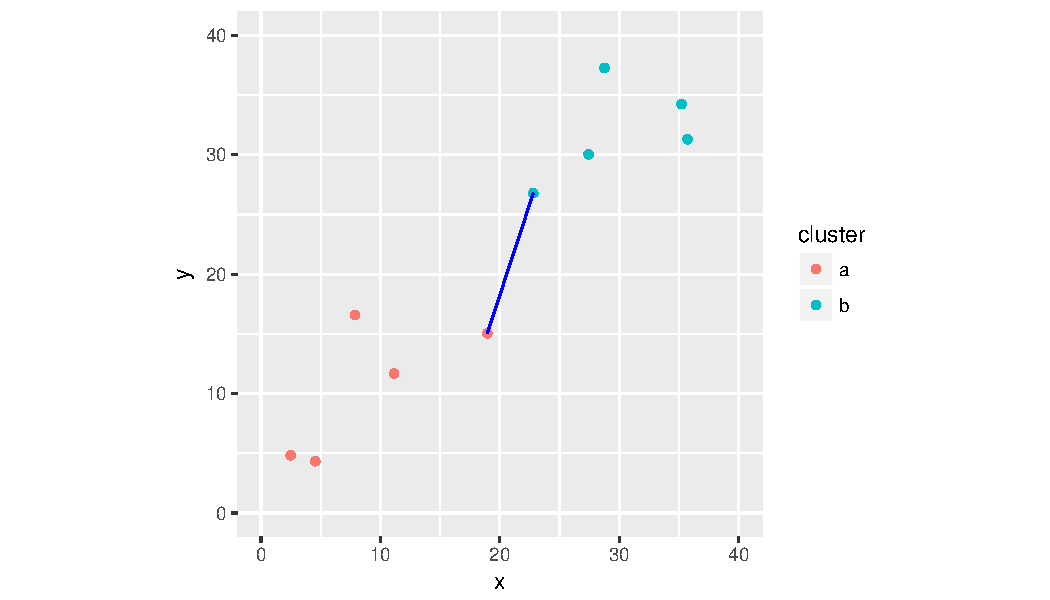
\includegraphics[width=\maxwidth]{figure/unnamed-chunk-3-1} 

\end{knitrout}
  
\end{frame}

\begin{frame}[fragile]{Better histogram}
  
  Set number of bins to 10:
  
\begin{knitrout}
\definecolor{shadecolor}{rgb}{0.969, 0.969, 0.969}\color{fgcolor}\begin{kframe}
\begin{alltt}
\hlkwd{ggplot}\hlstd{(drp,}\hlkwd{aes}\hlstd{(}\hlkwc{x}\hlstd{=score))}\hlopt{+}\hlkwd{geom_histogram}\hlstd{(}\hlkwc{bins}\hlstd{=}\hlnum{10}\hlstd{)}
\end{alltt}
\end{kframe}
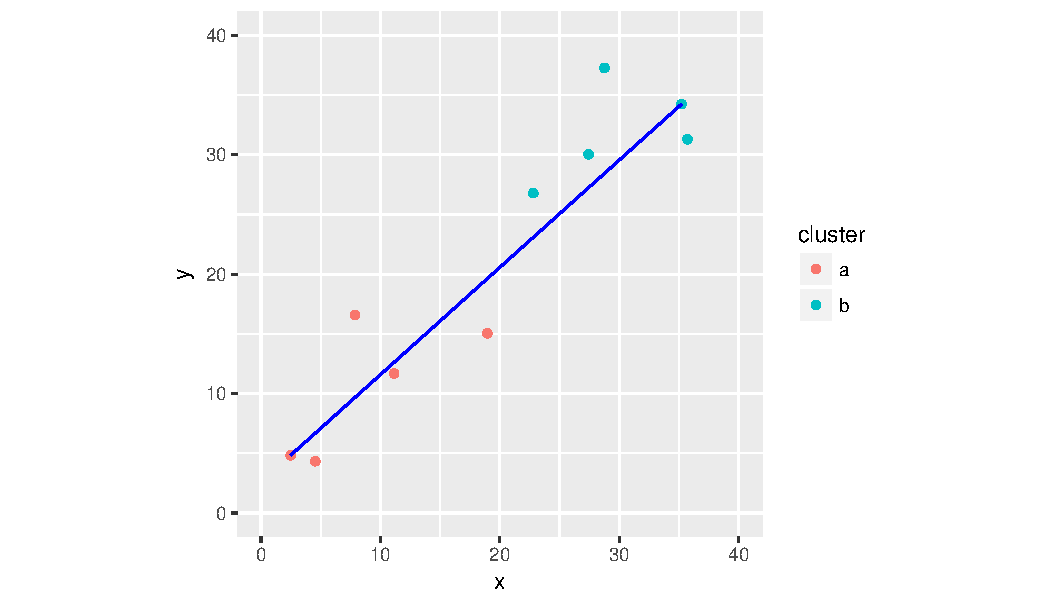
\includegraphics[width=\maxwidth]{figure/unnamed-chunk-4-1} 

\end{knitrout}
  
\end{frame}

\begin{frame}[fragile]{Histograms by group, side by side}
  
  Add a \texttt{facet\_grid}, thus:

\begin{knitrout}
\definecolor{shadecolor}{rgb}{0.969, 0.969, 0.969}\color{fgcolor}\begin{kframe}
\begin{alltt}
\hlkwd{ggplot}\hlstd{(drp,}\hlkwd{aes}\hlstd{(}\hlkwc{x}\hlstd{=score))}\hlopt{+}\hlkwd{geom_histogram}\hlstd{(}\hlkwc{bins}\hlstd{=}\hlnum{10}\hlstd{)}\hlopt{+}
  \hlkwd{facet_grid}\hlstd{(group}\hlopt{~}\hlstd{.)}
\end{alltt}
\end{kframe}
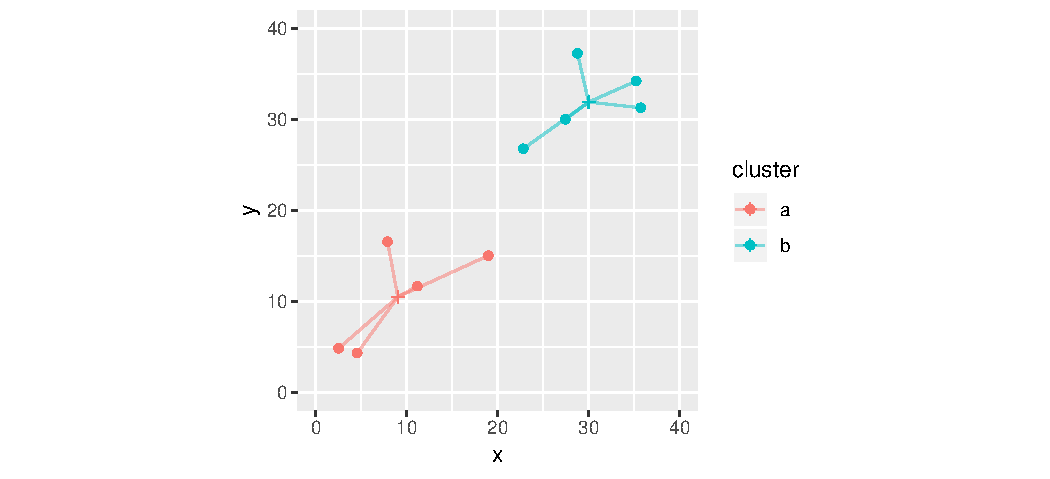
\includegraphics[width=\maxwidth]{figure/unnamed-chunk-5-1} 

\end{knitrout}
  
  
\end{frame}

\begin{frame}[fragile]{Comments}
  
  \begin{itemize}
  \item Control group scores (top) more spread out (they go higher
    and lower).
  \item Not sure how means/medians compare.
  \item Above/below histograms make for easier comparison.
  \item In \texttt{facet\_grid}, variable before squiggle denotes
    up/down, variable after squiggle denotes left/right (like
    \verb=y~x= in usual model formula).
  \item If nothing to go before or after squiggle, use \texttt{.}
    \begin{itemize}
    \item Here, no left-right graphs, so right side of squiggle is \texttt{.}
    \end{itemize}
  \end{itemize}
  
\end{frame}

\begin{frame}[fragile]{Boxplot of reading scores by group}

  Boxplot has $y$ scale (measured variable) \emph{and} $x$ scale
  (groups), so specify both:
  
\begin{knitrout}
\definecolor{shadecolor}{rgb}{0.969, 0.969, 0.969}\color{fgcolor}\begin{kframe}
\begin{alltt}
\hlkwd{ggplot}\hlstd{(drp,}\hlkwd{aes}\hlstd{(}\hlkwc{x}\hlstd{=group,}\hlkwc{y}\hlstd{=score))}\hlopt{+}\hlkwd{geom_boxplot}\hlstd{()}
\end{alltt}
\end{kframe}
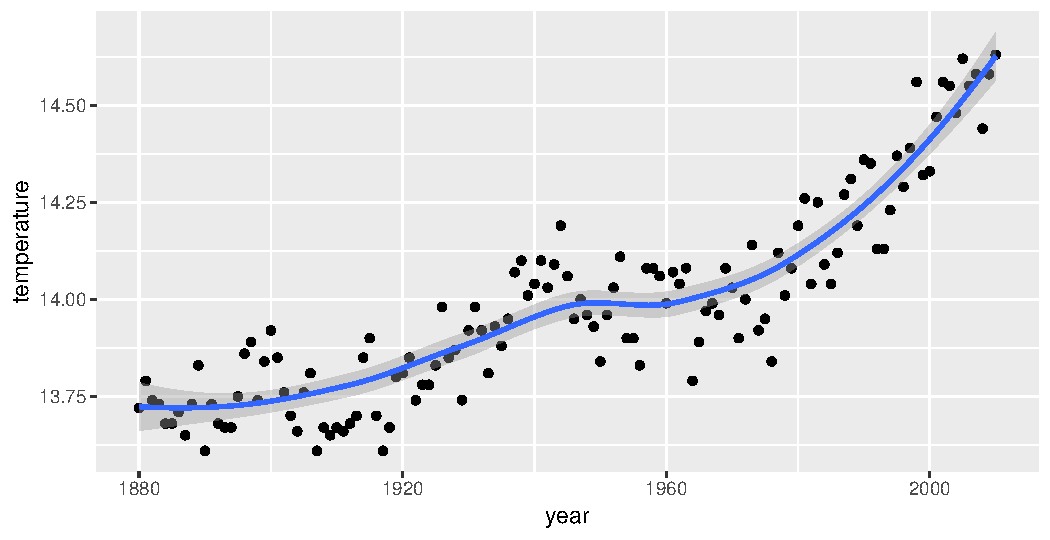
\includegraphics[width=\maxwidth]{figure/unnamed-chunk-6-1} 

\end{knitrout}
  
\end{frame}

\begin{frame}[fragile]{Boxplot of a single group}
  
  To get a boxplot of all the reading scores together, specify a
  ``dummy'' group for \texttt{x}:
  
\begin{knitrout}
\definecolor{shadecolor}{rgb}{0.969, 0.969, 0.969}\color{fgcolor}\begin{kframe}
\begin{alltt}
\hlkwd{ggplot}\hlstd{(drp,}\hlkwd{aes}\hlstd{(}\hlkwc{x}\hlstd{=}\hlkwd{factor}\hlstd{(}\hlnum{1}\hlstd{),}\hlkwc{y}\hlstd{=score))}\hlopt{+}\hlkwd{geom_boxplot}\hlstd{()}
\end{alltt}
\end{kframe}
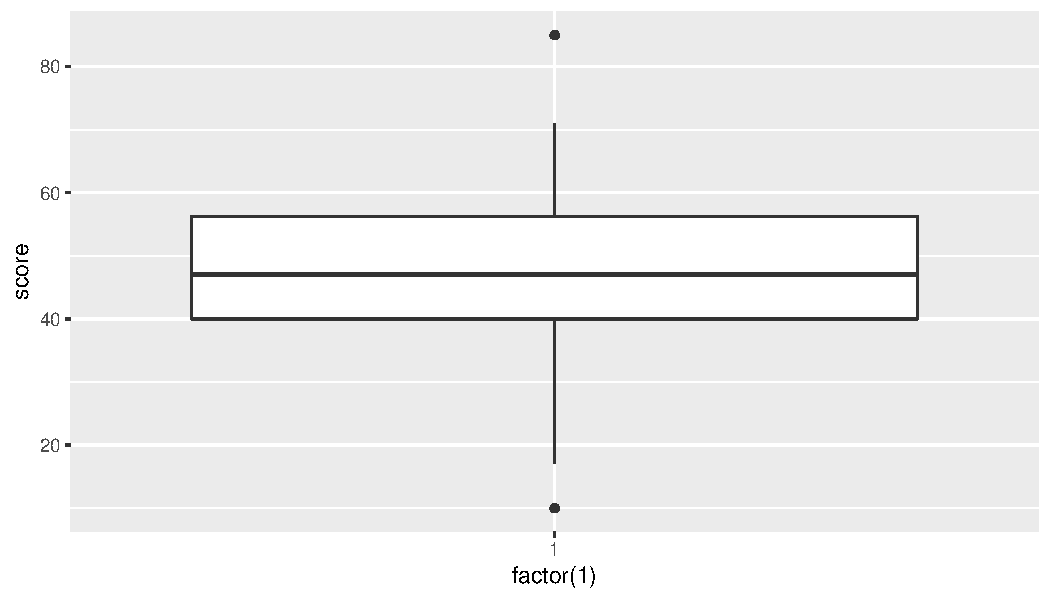
\includegraphics[width=\maxwidth]{figure/cateloupe-1} 

\end{knitrout}
  
\end{frame}

\begin{frame}[fragile]{Scatterplot}
  
For this, use analysis of covariance data from later:

\begin{knitrout}
\definecolor{shadecolor}{rgb}{0.969, 0.969, 0.969}\color{fgcolor}\begin{kframe}
\begin{alltt}
\hlstd{prepost}\hlkwb{=}\hlkwd{read.table}\hlstd{(}\hlstr{"ancova.txt"}\hlstd{,}\hlkwc{header}\hlstd{=T)}
\hlkwd{str}\hlstd{(prepost)}
\end{alltt}
\begin{verbatim}
## 'data.frame':	20 obs. of  3 variables:
##  $ drug  : Factor w/ 2 levels "a","b": 1 1 1 1 1 1 1 1 1 1 ...
##  $ before: int  5 10 12 9 23 21 14 18 6 13 ...
##  $ after : int  20 23 30 25 34 40 27 38 24 31 ...
\end{verbatim}
\end{kframe}
\end{knitrout}

\begin{itemize}
\item 
20 subjects were randomized to one of two drugs \texttt{a} and
\texttt{b}.
\item Each subject had their before and after scores measured on
some test.
\item Want a scatterplot of after score against before score
labelled by drug.
\end{itemize}
  
\end{frame}

\begin{frame}[fragile]{Basic scatterplot}
  
\begin{knitrout}
\definecolor{shadecolor}{rgb}{0.969, 0.969, 0.969}\color{fgcolor}\begin{kframe}
\begin{alltt}
\hlkwd{ggplot}\hlstd{(prepost,}\hlkwd{aes}\hlstd{(}\hlkwc{x}\hlstd{=before,}\hlkwc{y}\hlstd{=after))}\hlopt{+}\hlkwd{geom_point}\hlstd{()}
\end{alltt}
\end{kframe}
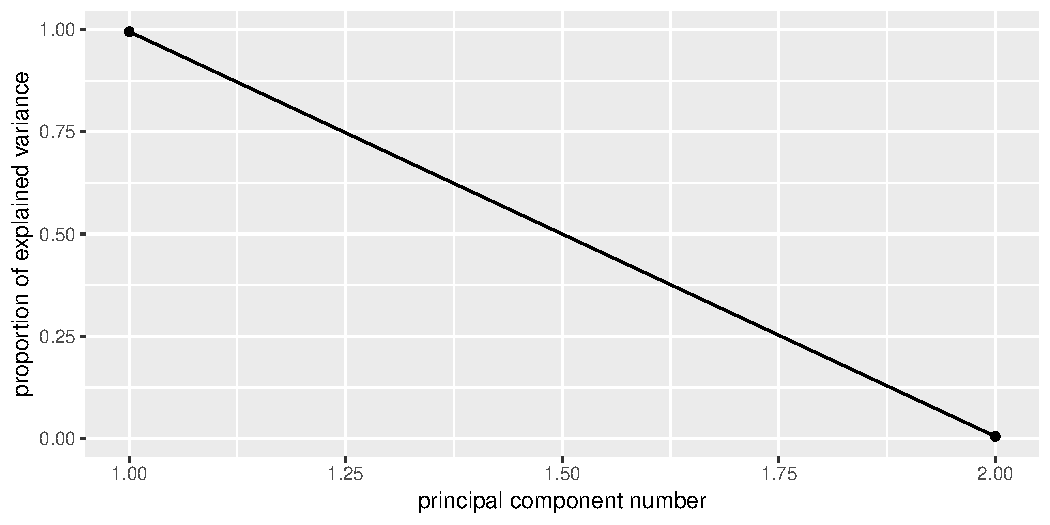
\includegraphics[width=\maxwidth]{figure/unnamed-chunk-8-1} 

\end{knitrout}
  
\end{frame}

\begin{frame}[fragile]{Coloured by \texttt{drug}}
  
Add \texttt{colour=} to the \emph{aesthetic}:

\begin{knitrout}
\definecolor{shadecolor}{rgb}{0.969, 0.969, 0.969}\color{fgcolor}\begin{kframe}
\begin{alltt}
\hlkwd{ggplot}\hlstd{(prepost,}\hlkwd{aes}\hlstd{(}\hlkwc{x}\hlstd{=before,}\hlkwc{y}\hlstd{=after,}\hlkwc{colour}\hlstd{=drug))}\hlopt{+}
  \hlkwd{geom_point}\hlstd{()}
\end{alltt}
\end{kframe}
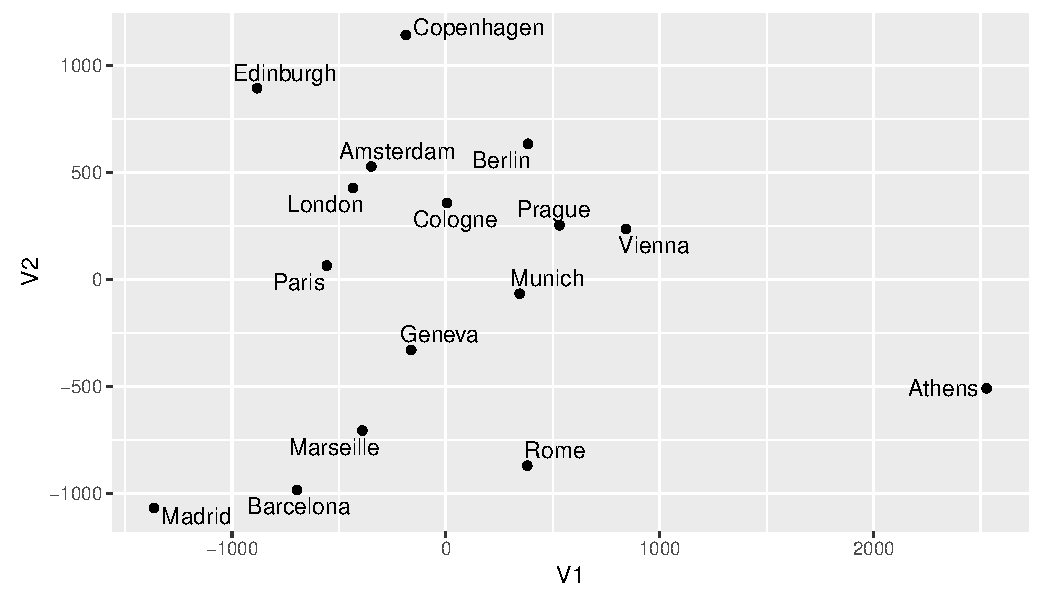
\includegraphics[width=\maxwidth]{figure/unnamed-chunk-9-1} 

\end{knitrout}
  
\end{frame}

\begin{frame}[fragile]{Adding a smooth trend}
  
\begin{knitrout}
\definecolor{shadecolor}{rgb}{0.969, 0.969, 0.969}\color{fgcolor}\begin{kframe}
\begin{alltt}
\hlkwd{ggplot}\hlstd{(prepost,}\hlkwd{aes}\hlstd{(}\hlkwc{x}\hlstd{=before,}\hlkwc{y}\hlstd{=after))}\hlopt{+}
  \hlkwd{geom_point}\hlstd{()}\hlopt{+}\hlkwd{geom_smooth}\hlstd{()}
\end{alltt}


{\ttfamily\noindent\itshape\color{messagecolor}{\#\# `geom\_smooth()` using method = 'loess'}}\end{kframe}
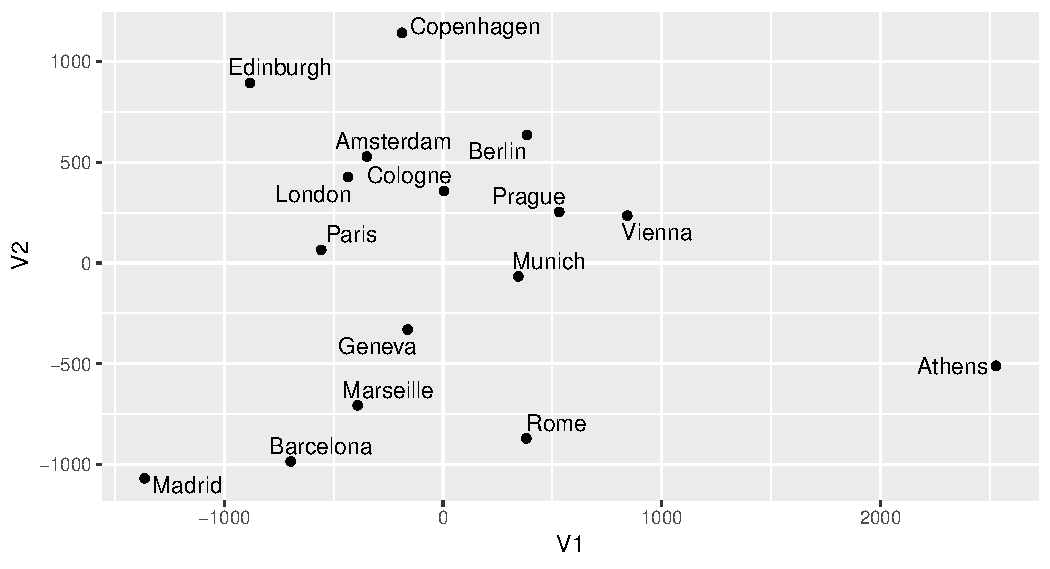
\includegraphics[width=\maxwidth]{figure/unnamed-chunk-10-1} 

\end{knitrout}
  
\end{frame}

\begin{frame}[fragile]{A smooth trend for each drug}
  
\begin{knitrout}
\definecolor{shadecolor}{rgb}{0.969, 0.969, 0.969}\color{fgcolor}\begin{kframe}
\begin{alltt}
\hlkwd{ggplot}\hlstd{(prepost,}\hlkwd{aes}\hlstd{(}\hlkwc{x}\hlstd{=before,}\hlkwc{y}\hlstd{=after,}\hlkwc{colour}\hlstd{=drug))}\hlopt{+}
  \hlkwd{geom_point}\hlstd{()}\hlopt{+}\hlkwd{geom_smooth}\hlstd{()}
\end{alltt}


{\ttfamily\noindent\itshape\color{messagecolor}{\#\# `geom\_smooth()` using method = 'loess'}}\end{kframe}
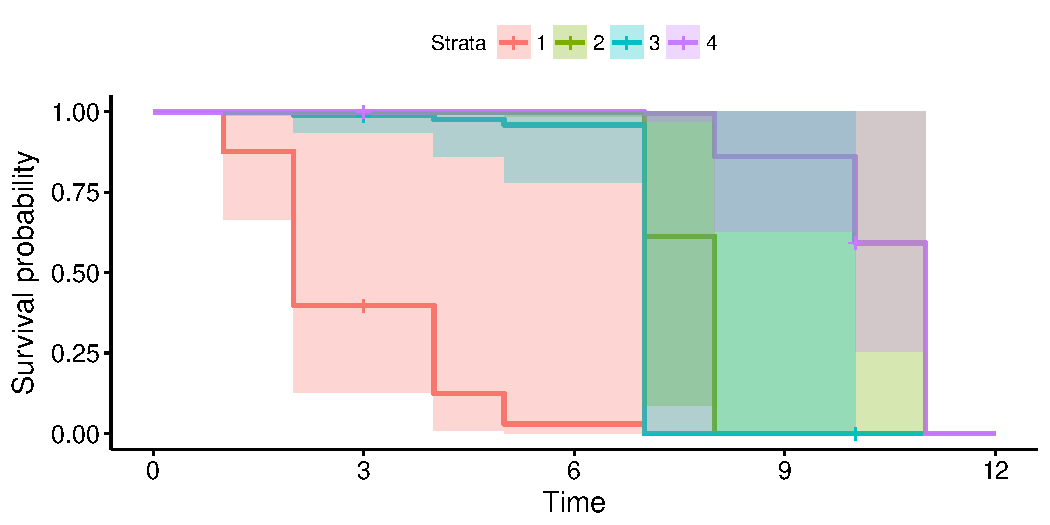
\includegraphics[width=\maxwidth]{figure/unnamed-chunk-11-1} 

\end{knitrout}
  
\end{frame}

\begin{frame}[fragile]{A regression line}

\begin{knitrout}
\definecolor{shadecolor}{rgb}{0.969, 0.969, 0.969}\color{fgcolor}\begin{kframe}
\begin{alltt}
\hlkwd{ggplot}\hlstd{(prepost,}\hlkwd{aes}\hlstd{(}\hlkwc{x}\hlstd{=before,}\hlkwc{y}\hlstd{=after))}\hlopt{+}
  \hlkwd{geom_point}\hlstd{()}\hlopt{+}\hlkwd{geom_smooth}\hlstd{(}\hlkwc{method}\hlstd{=}\hlstr{"lm"}\hlstd{)}
\end{alltt}
\end{kframe}
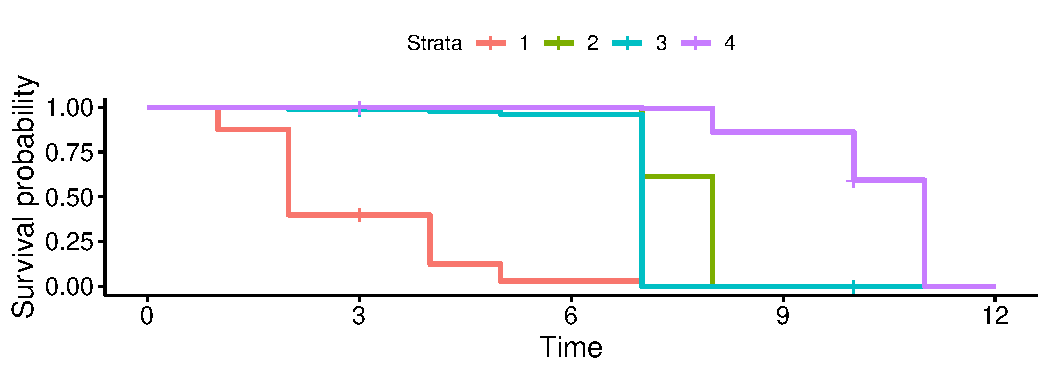
\includegraphics[width=\maxwidth]{figure/unnamed-chunk-12-1} 

\end{knitrout}
  
  
  
\end{frame}

\begin{frame}[fragile]{A regression line for each drug}

\begin{knitrout}
\definecolor{shadecolor}{rgb}{0.969, 0.969, 0.969}\color{fgcolor}\begin{kframe}
\begin{alltt}
\hlkwd{ggplot}\hlstd{(prepost,}\hlkwd{aes}\hlstd{(}\hlkwc{x}\hlstd{=before,}\hlkwc{y}\hlstd{=after,}\hlkwc{colour}\hlstd{=drug))}\hlopt{+}
  \hlkwd{geom_point}\hlstd{()}\hlopt{+}\hlkwd{geom_smooth}\hlstd{(}\hlkwc{method}\hlstd{=}\hlstr{"lm"}\hlstd{)}
\end{alltt}
\end{kframe}
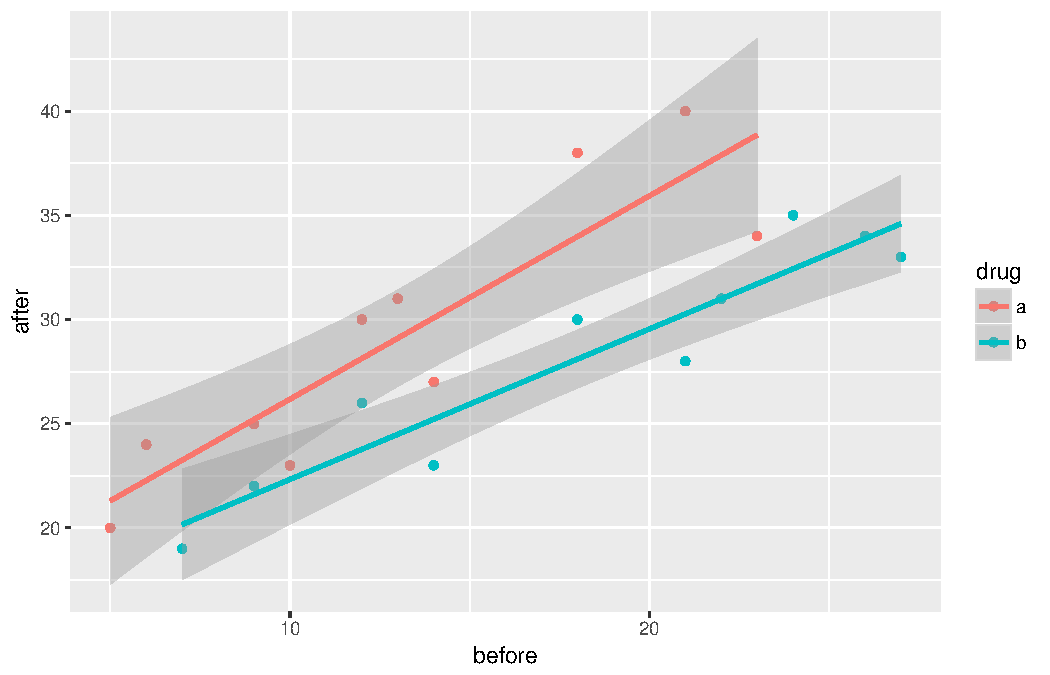
\includegraphics[width=\maxwidth]{figure/kalloni-1} 

\end{knitrout}
  
\end{frame}



\begin{frame}[fragile]{Think of before-after data as repeated measures}
  
  Reorganize:
  
\begin{knitrout}
\definecolor{shadecolor}{rgb}{0.969, 0.969, 0.969}\color{fgcolor}\begin{kframe}
\begin{alltt}
\hlstd{prepost} \hlopt \hlkwd{mutate}\hlstd{(}\hlkwc{subject}\hlstd{=}\hlkwd{row_number}\hlstd{())} \hlopt
  \hlkwd{gather}\hlstd{(time,score,before}\hlopt{:}\hlstd{after,}
  \hlkwc{factor_key}\hlstd{=T)} \hlkwb{->} \hlstd{prepost.long}
\hlstd{prepost.long} \hlopt \hlkwd{sample_n}\hlstd{(}\hlnum{8}\hlstd{)} \hlcom{# 8 random rows}
\end{alltt}
\begin{verbatim}
##    drug subject   time score
## 5     a       5 before    23
## 6     a       6 before    21
## 16    b      16 before    22
## 33    b      13  after    33
## 37    b      17  after    34
## 20    b      20 before     9
## 10    a      10 before    13
## 9     a       9 before     6
\end{verbatim}
\end{kframe}
\end{knitrout}

\emph{One} column of scores, with column \texttt{time} saying whether
was before or after.
  
\end{frame}

\begin{frame}[fragile]{A ``spaghetti plot''}
  
\begin{knitrout}
\definecolor{shadecolor}{rgb}{0.969, 0.969, 0.969}\color{fgcolor}\begin{kframe}
\begin{alltt}
\hlkwd{ggplot}\hlstd{(prepost.long,}\hlkwd{aes}\hlstd{(}\hlkwc{x}\hlstd{=time,}\hlkwc{y}\hlstd{=score,}\hlkwc{colour}\hlstd{=drug,}
  \hlkwc{group}\hlstd{=subject))}\hlopt{+}\hlkwd{geom_point}\hlstd{()}\hlopt{+}\hlkwd{geom_line}\hlstd{()}
\end{alltt}
\end{kframe}
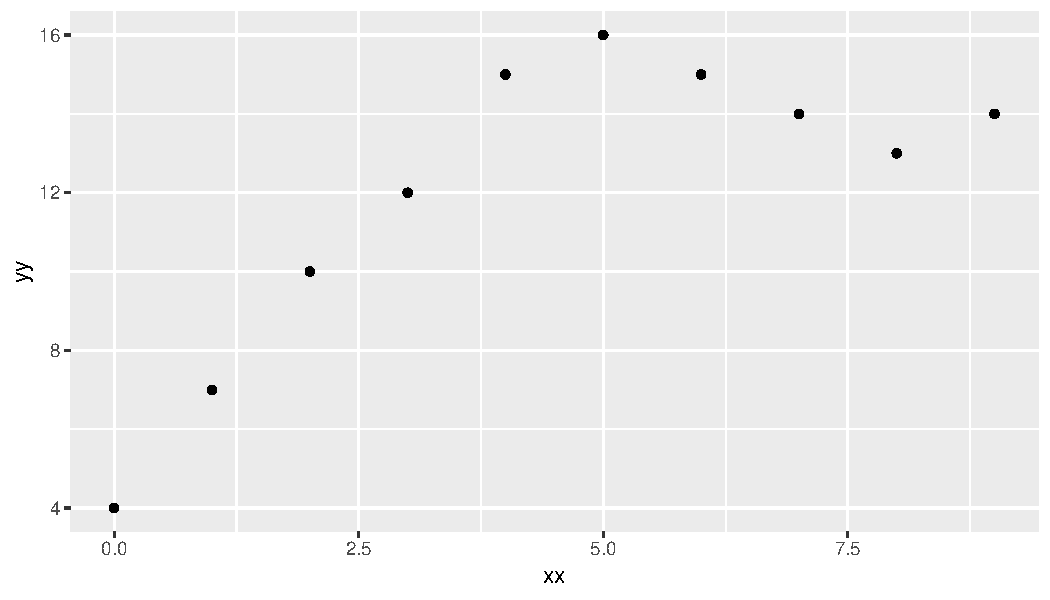
\includegraphics[width=\maxwidth]{figure/unnamed-chunk-14-1} 

\end{knitrout}
  
\end{frame}

\begin{frame}[fragile]{Exponential growth data}
  
  \begin{itemize}
  \item I made up these data:
\begin{knitrout}
\definecolor{shadecolor}{rgb}{0.969, 0.969, 0.969}\color{fgcolor}\begin{kframe}
\begin{alltt}
\hlstd{x}\hlkwb{=}\hlnum{0}\hlopt{:}\hlnum{5}
\hlstd{y}\hlkwb{=}\hlkwd{c}\hlstd{(}\hlnum{2.0}\hlstd{,}\hlnum{4.1}\hlstd{,}\hlnum{8.2}\hlstd{,}\hlnum{15.8}\hlstd{,}\hlnum{31.6}\hlstd{,}\hlnum{65.0}\hlstd{)}
\hlstd{grow}\hlkwb{=}\hlkwd{data.frame}\hlstd{(x,y)}
\hlstd{grow}
\end{alltt}
\begin{verbatim}
##   x    y
## 1 0  2.0
## 2 1  4.1
## 3 2  8.2
## 4 3 15.8
## 5 4 31.6
## 6 5 65.0
\end{verbatim}
\end{kframe}
\end{knitrout}

\item Each $y$-value is approximately twice as big as the previous:
  exponential growth.
  \end{itemize}
  
\end{frame}

\begin{frame}[fragile]{Scatter plot with line (bad)}
  
\begin{knitrout}
\definecolor{shadecolor}{rgb}{0.969, 0.969, 0.969}\color{fgcolor}\begin{kframe}
\begin{alltt}
\hlkwd{ggplot}\hlstd{(grow,}\hlkwd{aes}\hlstd{(}\hlkwc{x}\hlstd{=x,}\hlkwc{y}\hlstd{=y))}\hlopt{+}
  \hlkwd{geom_point}\hlstd{()}\hlopt{+}\hlkwd{geom_smooth}\hlstd{(}\hlkwc{method}\hlstd{=}\hlstr{"lm"}\hlstd{)}
\end{alltt}
\end{kframe}
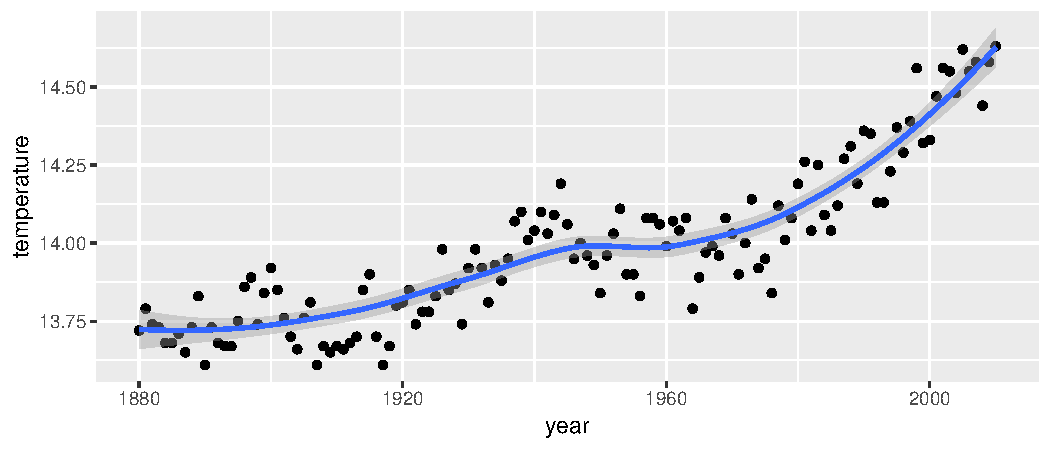
\includegraphics[width=\maxwidth]{figure/unnamed-chunk-16-1} 

\end{knitrout}
  
\end{frame}

\begin{frame}[fragile]{Use log scale for $y$-axis}

\begin{knitrout}
\definecolor{shadecolor}{rgb}{0.969, 0.969, 0.969}\color{fgcolor}\begin{kframe}
\begin{alltt}
\hlkwd{ggplot}\hlstd{(grow,}\hlkwd{aes}\hlstd{(}\hlkwc{x}\hlstd{=x,}\hlkwc{y}\hlstd{=y))}\hlopt{+}
  \hlkwd{geom_point}\hlstd{()}\hlopt{+}\hlkwd{coord_trans}\hlstd{(}\hlkwc{y}\hlstd{=}\hlstr{"log10"}\hlstd{)}
\end{alltt}
\end{kframe}
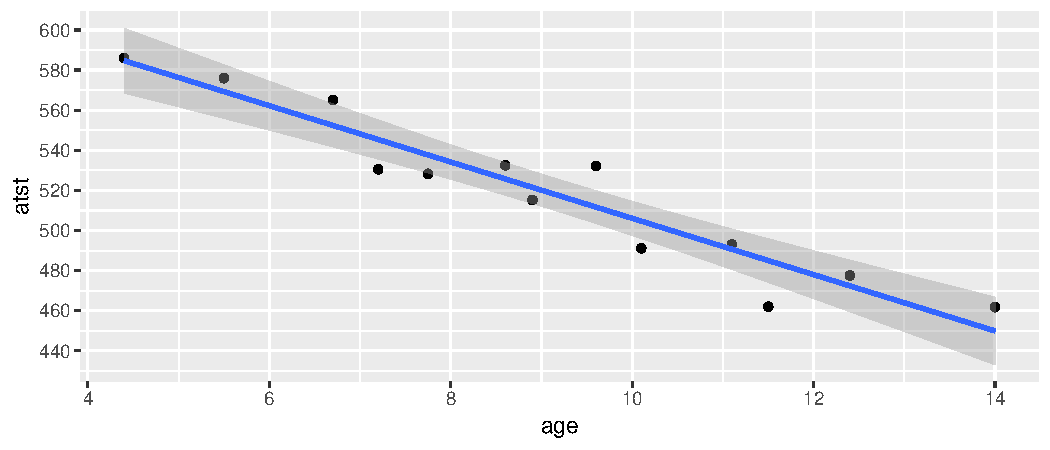
\includegraphics[width=\maxwidth]{figure/unnamed-chunk-17-1} 

\end{knitrout}

On this plot, trend is straight.

\end{frame}
